\subsection{分类问题}

此问题中数据来源为手写数字图片生成的灰度矩阵, 目标为将手写的数字分类为``0''到``9''.

对于该问题采用四层全连接层, 前三层采用ReLU激活, 输出层采用softmax激活.
采用与softmax函数匹配的交叉熵作为损失函数. 学习率设置为0.005, 每次训练
都随机从训练集中抽取100个数据进行训练以防止过拟合.

经过几次测试, 分类准确率平均达到96\%以上, 损失函数随训练次数变化情况如图所示:

\begin{figure}[H]
    \centering
    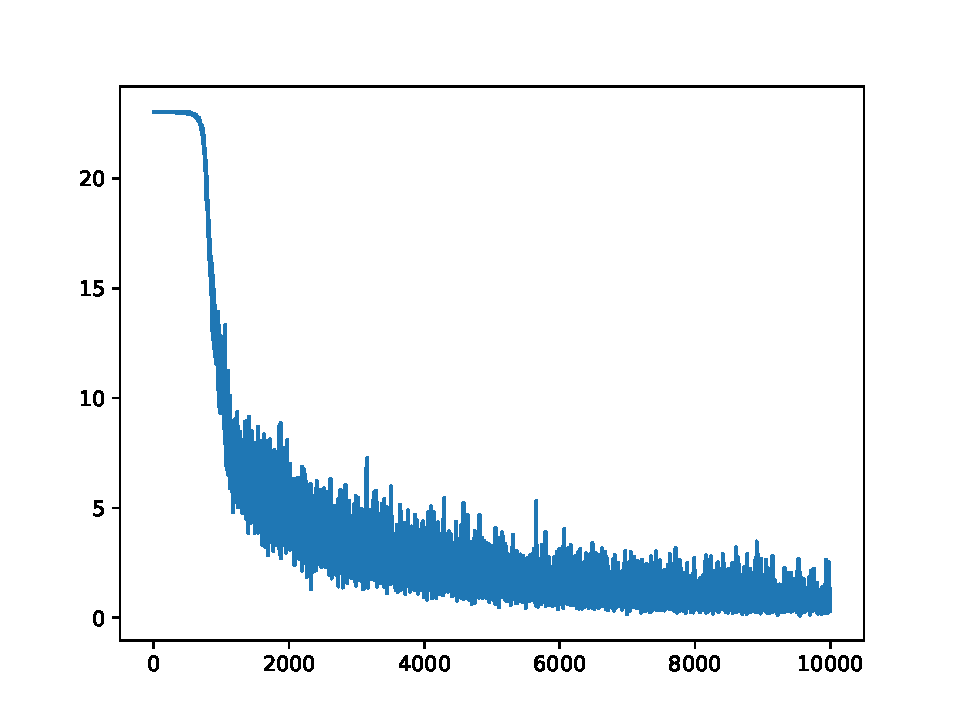
\includegraphics[width=0.7\textwidth]{figures/classification.pdf}
    \caption{交叉熵损失函数随训练次数的变化情况}
\end{figure}

\subsection{回归问题}

此问题的数据来自于一个房屋面积、房间数量以及房价的表格, 根据这些数据回归拟合
房价关于房屋面积以及房间数量的二元函数.

对于该问题采用两层全连接层, 第一层采用ReLU激活, 第二层直接输出.
采用SME函数作为损失函数. 学习率设置为0.01, 每次训练都随机抽取10个数据.

以下是损失函数下降情况以及拟合函数的图像.

\begin{figure}[H]
    \centering
    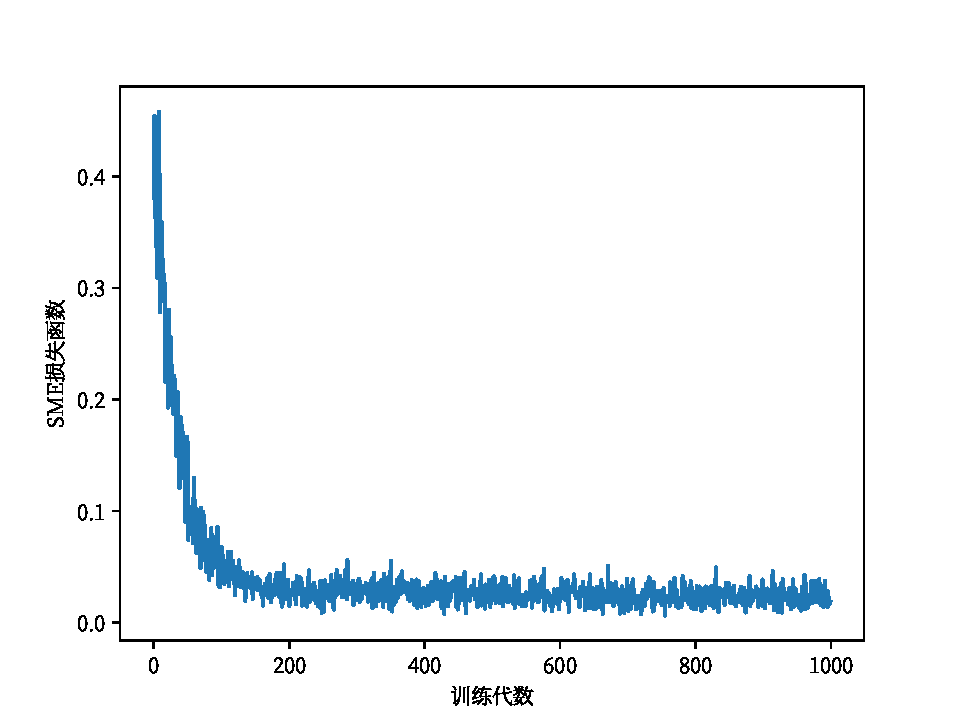
\includegraphics[width=0.7\textwidth]{figures/regress-epoch.pdf}
    \caption{SME损失函数随训练次数的变化情况}
\end{figure}

\begin{figure}[H]
    \centering
    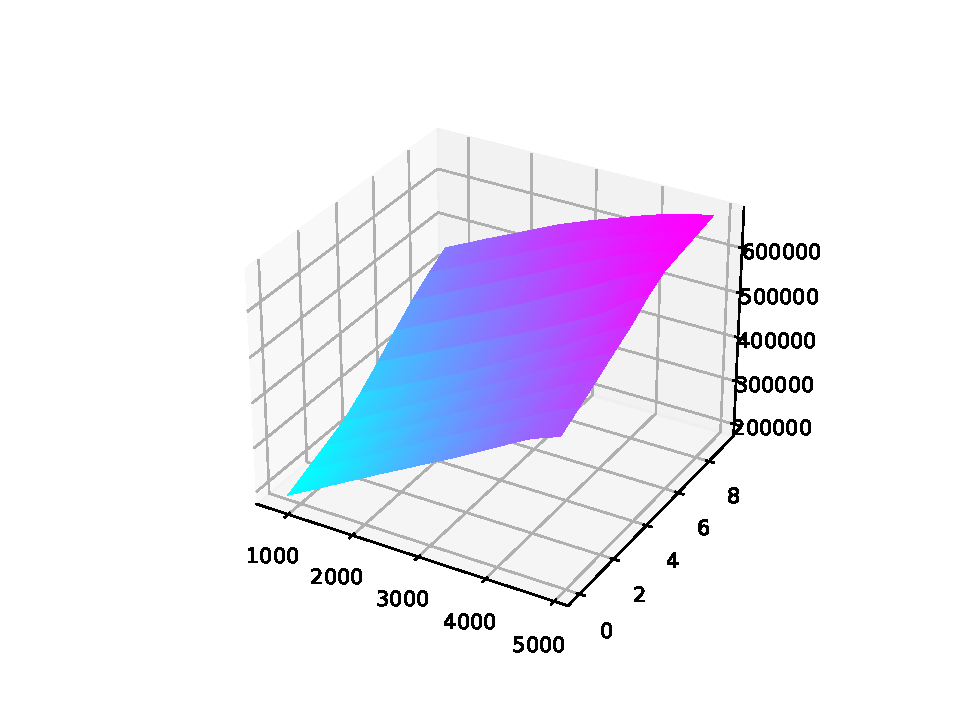
\includegraphics[width=0.9\textwidth]{figures/regress.pdf}
    \caption{房价回归预测函数示意图}
\end{figure}